\chapter{Felhasználói dokumentáció} % User guide
\label{ch:user}

\section{A feladat ismertetése}

\begin{figure}[H]
	\centering
	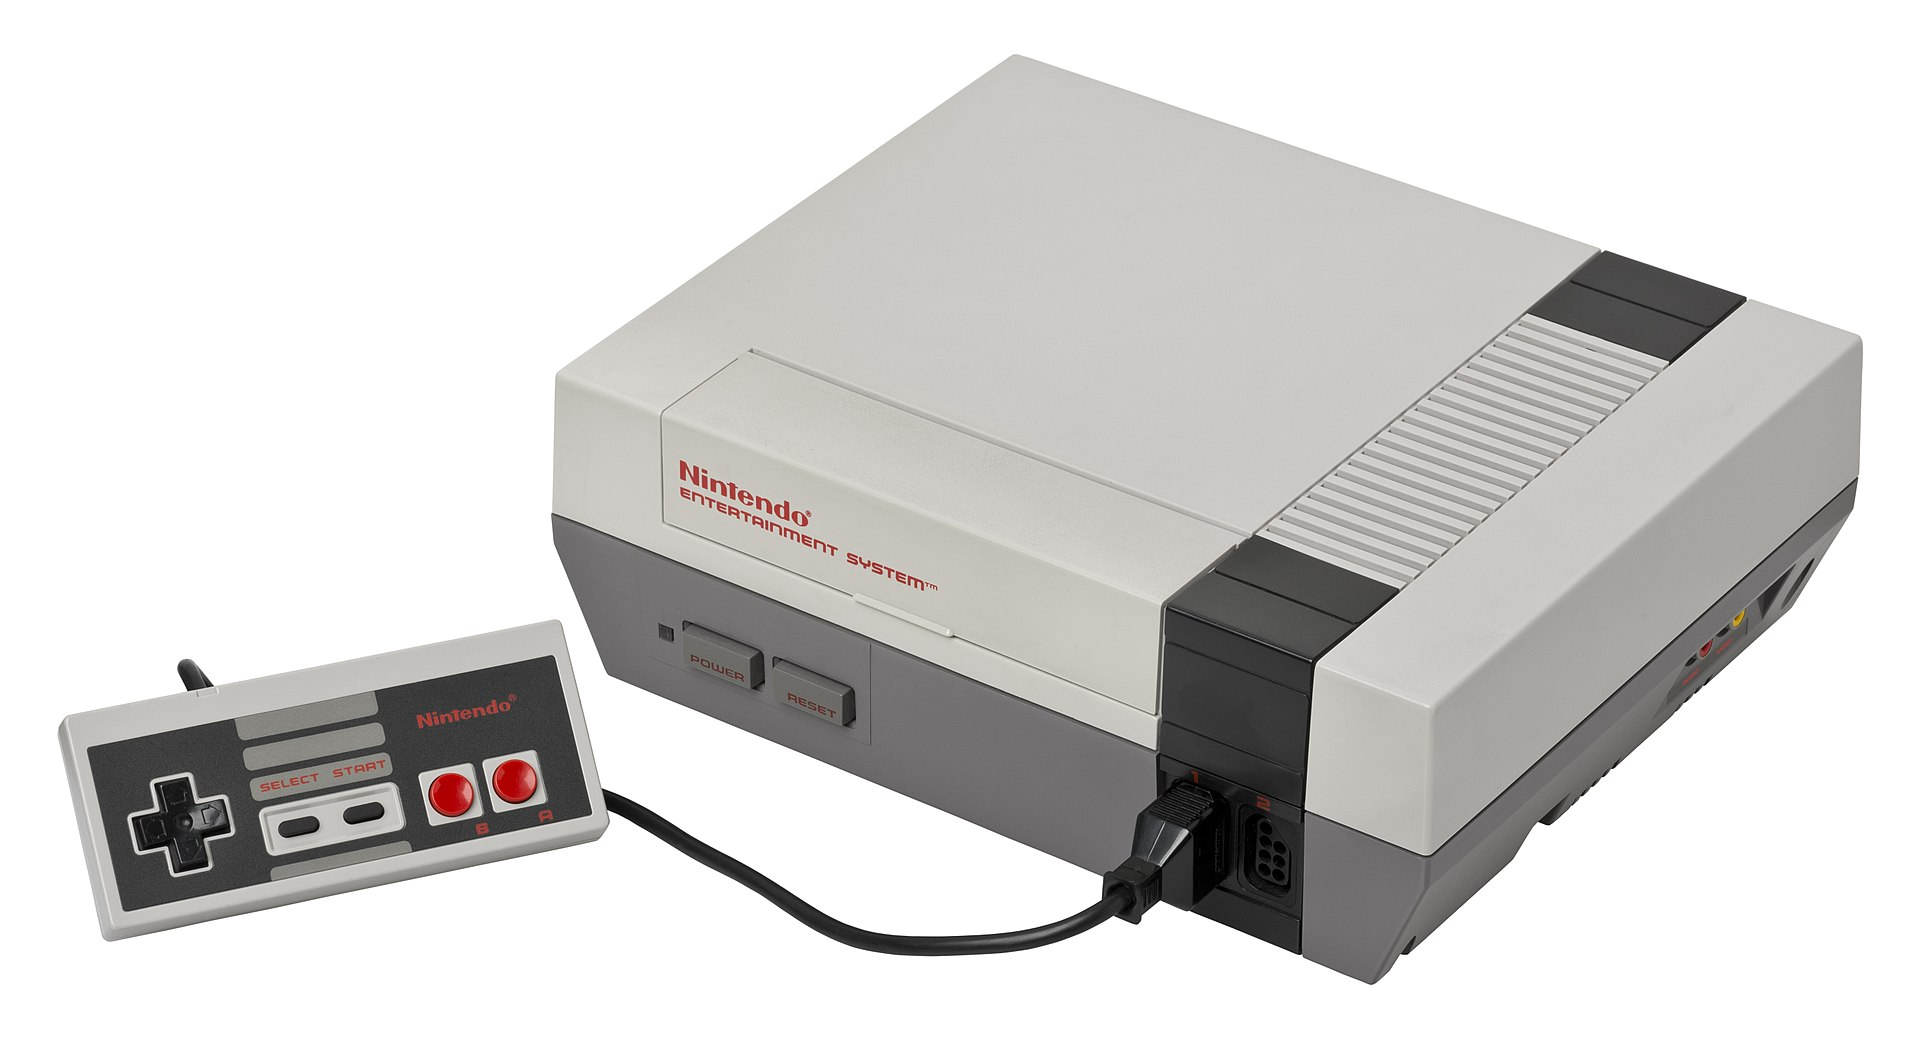
\includegraphics[scale=0.16]{nes.jpg}
	\caption{Nintendo Entertainment System (1985)\protect\footnotemark}
	\label{fig:nes}
\end{figure}

\footnotetext{\url{https://upload.wikimedia.org/wikipedia/commons/8/82/Nintendo-Entertainment-System-NES-Console-FL.jpg}}
A program feladata a NES kazetták futtatása. A felhasználó grafikus felület segítségével kiválaszthatja a futtatni kívánt, iNES formátumú kazetta fájlt, majd annak betöltése után az emulátor belekezd a videókimenet előállításába.\footnote{A hangfeldolgozást nem emulálja a program} Bemeneti eszközként billentyűzet vagy kontroller használható. A futtatás során lehetőség van az emulátor állapotának fájlként való mentésére és betöltésére. Az emulációt többféle módon is befolyásolhatja a felhasználó, amikbe beletartozik a játék szüneteltetése, adott mennyiségű CPU utasítás végrehajtása, valamint a teljes képkockánként történő léptetés.

A programot azoknak ajánlom, akik egy letisztult kezelőfelülettel rendelkező, több platformon is elérhető NES emulátorral szeretnék játszani kedvenc játékaikat.

\section{Minimum rendszerkövetelmények}

\begin{description}
	\item[Processzor:] Intel Core 2 Duo E8400 @ 3.0 GHz
	\item[Memória:] 2 GB DDR2 @ 800 MHz
	\item[Videókártya:] OpenGL 4.3 kompatibilis videókártya
	\item[Tárhely:] 161 MB
	\item[Operációs rendszer:] Linux, Windows
\end{description}

A program a fenti konfiguráción történő tesztelés során problémamentesen működött.

\section{Telepítés}

\begin{itemize}
	\item Windows: A programot egy telepítőfájl segítségével telepíthetjük.
	\item Linux:
	\begin{lstlisting}[language=bash]
	$ tar xvf pure-nes-1.0.tar.gz
	$ cd pure-nes-1.0
	$ ./configure
	$ make
	\end{lstlisting}
\end{itemize}

\section{Indítás}
\begin{itemize}
	\item Windows: Kattintsunk a program parancsikonjára a Start Menüben vagy az asztalon.
	\item Linux:
	\begin{lstlisting}[language=bash]
	pure-nes-1.0$ stack exec pure-nes
	\end{lstlisting}
\end{itemize}


\section{Kompatibilis kazetták}

A NES megtervezésekor fontos cél volt, hogy a konzol életciklusa hosszú legyen, de ezt nem volt könnyű gazdaságos módon elérni. Azt a megoldás találták ki, hogy a kazetta a játék mellett tartalmazzon speciális integrált áramköröket, amik igény szerint bővíthették a hardveres erőforrásokat. A kiegészítőegységek egy konkrét összeállítását \emph{mapper}-nek nevezzük. A későbbi játékok előszeretettel használták ki ezt a lehetőséget. A legtöbb speciális áramkör a megnövelt háttértár kezeléséhez volt szükséges, de akadt olyan is, amelyik további hangcsatornákat adott hozzá a hangfeldolgozó egységhez. Az emulátorom jelenleg a 0, 2 és 3 azonosítójú mapper-eket használó kazettákat támogatja, ezáltal 471 játékot képes elindítani. 

\section{Főmenü}

\begin{center}
	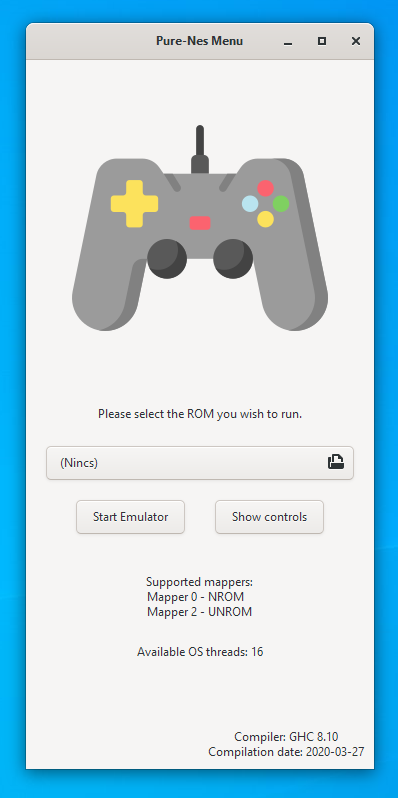
\includegraphics[scale=0.8]{menu.png}
\end{center}

\subsection{Kazetta kiválasztása}

A fájlkiválasztó segítségével adjuk meg a futtatni kívánt kazettát vagy mentést, majd nyomjunk a \emph{Start Emulator} gombra.
A program hibaüzenettel jelzi, ha a kazetta nem kompatibilis vagy a fájl formátuma nem megfelelő.

\subsection{Irányítási beállítások megtekintése}

A főmenü \emph{Show controls} gombjára kattintva megtekinthetjük a gombhozzárendeléseket.

\begin{center}
	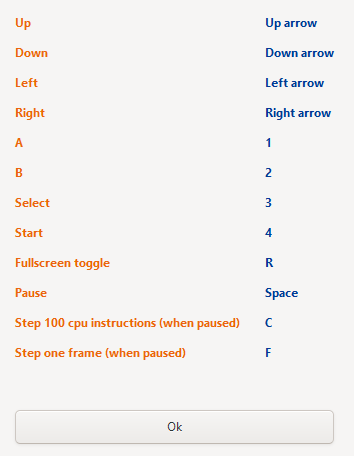
\includegraphics[scale=0.74]{controls.png}
\end{center}

\section{Játék alatt elérhető funkciók}

\begin{figure}[H]
	\centering
	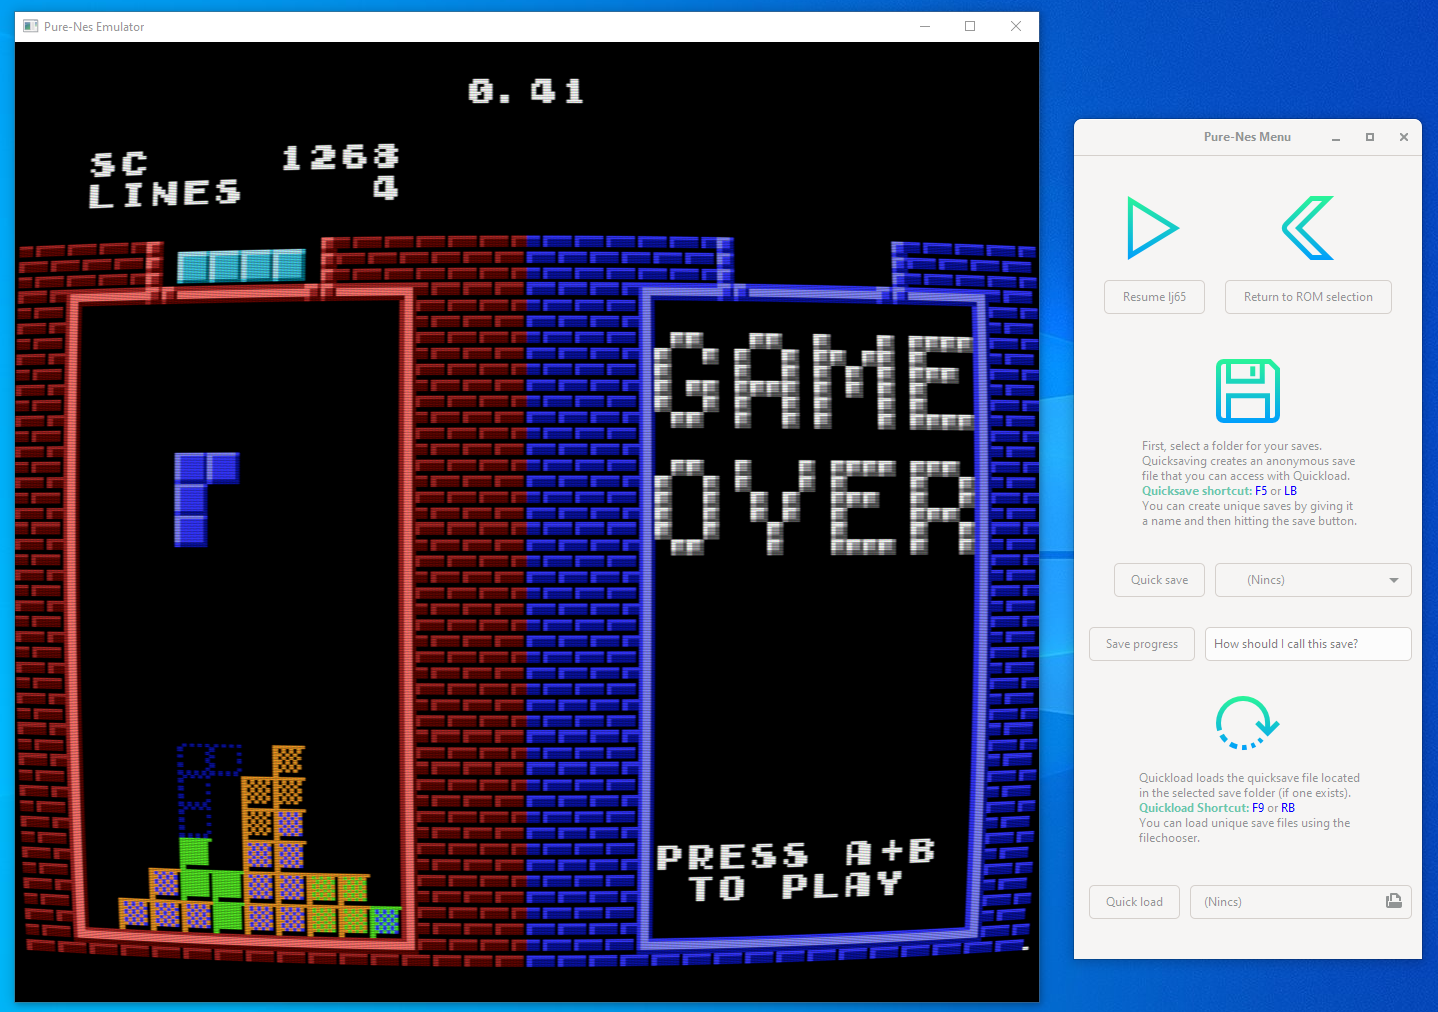
\includegraphics[scale=0.4]{tetris.png}
	\caption{A felhasználói felület játék közben\protect\footnotemark}
\end{figure}

\subsection {Irányítás}

\begin{table}[H]
	\centering
	\begin{tabular}{ | l |  l | l | }
		\hline
		NES kontroller gomb & Billentyű & Kontroller \\
		\hline			
		A      & 1 & 2. gomb \\
		B      & 2 & 3. gomb \\
		Select & 3 & 0. gomb \\
		Start  & 4 & 1. gomb \\
		Up     & Fel nyíl & DPad Fel \\
		Down   & Lefele nyíl & DPad Le \\
		Left   & Balra nyíl & DPad Bal \\ 
		Right  & Jobbra nyíl & DPad Jobb \\
		\hline
	\end{tabular}
	\caption{Játékok irányításához használt gombok}
	\label{fig:btns}
\end{table}
\footnotetext{Link a képen szereplő LJ65 játékhoz: \url{https://github.com/Glavin001/node-nes/tree/master/roms/lj65}}
A \ref{fig:btns} táblázatban látható módon vannak a fizikai gombok (a billentyűzeten vagy a kontrolleren) az emulált NES virtuális gombjainak megfeleltetve. Például, ha a játékon belül a \emph{Select} gombot szeretnénk lenyomni, akkor a billentyűzeten a 3-as, vagy a kontrolleren a 0. gombot kell lenyomnunk.
A Joystick vezérlők gombkiosztása el szokott térni, ami azt jelenti, hogy a fizikailag ugyanott található gomboknak más az azonosítója. A felhasználó feladata, hogy szükség esetén egy másik programmal módosítsa eszközének kiosztását úgy, hogy az megegyezzen az emulátor szerint elvárttal.

Az \ref{fig:emucontrol} táblázatban felsorolt gombokkal lehet az emulációt irányítani és testre szabni. A szüneteltetés leállítja az emulált komponenseket és elérhetővé teszi a léptetési funkciókat. Képesek vagyunk a teljes rendszert egy processzorutasítással léptetni. Minden léptetésnél láthatjuk a sztenderd kimeneten, hogy milyen utasítások fognak soron következni. Ha ennél gyorsabb ütemben szeretnénk léptetni az emulációt, akkor használjuk a képkockánti léptetést. A képre alapértelmezetten rákerül egy katódsugárcsöves megjelenítőket szimuláló effektus, de ezt a funkciót bármikor kikapcsolhatjuk.

\begin{table}[H]
	\centering
	\begin{tabular}{ | l | c | }
		\hline
		Emulátor funkció & Billentyű \\
		\hline			
		Teljes képernyős nézet ki/be & R \\
		Katódsugárcsöves képernyő-effektus ki/be & T \\
		Szüneteltetés ki/be & Space \\
		Egy processzorutasítás végrehajtása (szüneteltetés alatt) & C \\
		Léptetés a következő képkockára (szüneteltetés alatt) & F \\
		\hline
	\end{tabular}
	\caption{Az emuláció vezérlése}
	\label{fig:emucontrol}
\end{table}

\subsection{Mentés}

A felhasználónak ki kell jelölnie egy mappát, amit a program a mentések kezelésére használ. A program hibaüzenetet ad, ha enélkül próbálunk menteni vagy gyors betöltést végrehajtani.

A mentések a virtuális gép teljes állapota mellett a praktikusság érdekében a játék másolatát is tartalmazzák, tehát egy mentés betöltéséhez nem kell megőrizni a játék eredeti példányát.

\begin{center}
	
\includegraphics[scale=0.75]{save.png}
\end{center}

\subsubsection{Gyorsmentés}

A gyorsmentési funkcióval egy gombnyomásra elmenthetjük állásunkat. A mentés \emph{quick.purenes} néven jön létre a mappában. Ha már létezik ilyen fájl, az felül lesz írva.
Mentés létrehozása: \textbf{Quicksave} gomb vagy \textbf{F5} billentyű vagy a \textbf{4.} gomb a kontrolleren.
A mentés sikerességét egy pipa vagy kereszt jelzi a kezelőfelületen a mentés ikon mellett.
Ha a kontroller rendelkezik rezgőmotorral, akkor a sikeres mentés rezgéssel is jelezve lesz.

\subsubsection{Egyedi mentés létrehozása}

Adhatunk nevet a mentéseknek, ehhez írjuk be a nevet a szövegmezőbe és nyomjunk a \emph{Save} gombra. A mentés \emph{\{név\}.purenes} néven jön létre a mappában. A \emph{quick} nevet nem adhatjuk a mentésnek.

\subsection{Betöltés}

\subsubsection{Gyorsbetöltés}

A gyorsbetöltési funkció játék közben érhető el, miután kiválasztottuk a mentéseket tároló mappát. A \textbf{Quickload} gombbal, vagy az \textbf{F9} billentyűvel, vagy a kontroller \textbf{6.} gombjával visszatölthetjük a korábban létrehozott gyorsmentést.
A betöltés sikeressége a mentéshez hasonló módon jelenik meg a kezelőfelületen.
Sikertelen betöltés abból adódhat, hogy a mappában nem található gyorsmentés, vagy a mentési fájl sérült.
A sikeres betöltést itt is rezgés fogja követni.

\begin{center}
	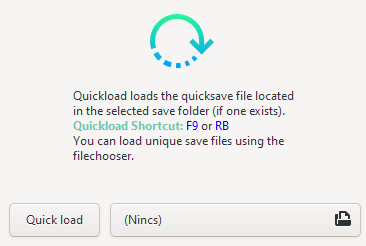
\includegraphics[scale=0.75]{load.png}
\end{center}


\begin{subsubsection}{Egyedi mentés betöltése}

Ez a funkció arra szolgál, hogy a gyorsmentésen kívül más mentéseket is be tudjunk tölteni. A fájlkiválasztó segítségével válasszuk ki a betölteni kívánt mentést. \newline \textbf{Figyelem:} Mindkét betöltési módnál az aktuális munkamenet elveszik. Ha ezt el szeretnénk kerülni, akkor mentsünk előtte.

\end{subsubsection}

\subsection{A játék megállítása}

A játék futása bármikor felfüggeszthető a \emph{Pause} gombbal, majd ezután folytatható a \emph{Resume} gombbal.

\begin{center}
	
\includegraphics[scale=0.8]{pause.png}
	\qquad
	
\includegraphics[scale=0.8]{resume.png}
\end{center}

\subsection{Visszatérés a főmenübe}
A \emph{Return To ROM selection} gomb bezárja a játékot és a felhasználói felületen visszanavigál minket a főmenübe.
\newline \textbf{Figyelem:} Az állásunk elveszik, ha előtte nem mentünk. 
\vspace{0.3cm}
\begin{center}
	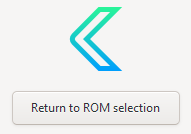
\includegraphics[scale=0.8]{return.png}
\end{center}

\subsection{Képernyőképek}
\begin{figure}[H]
	\centering
	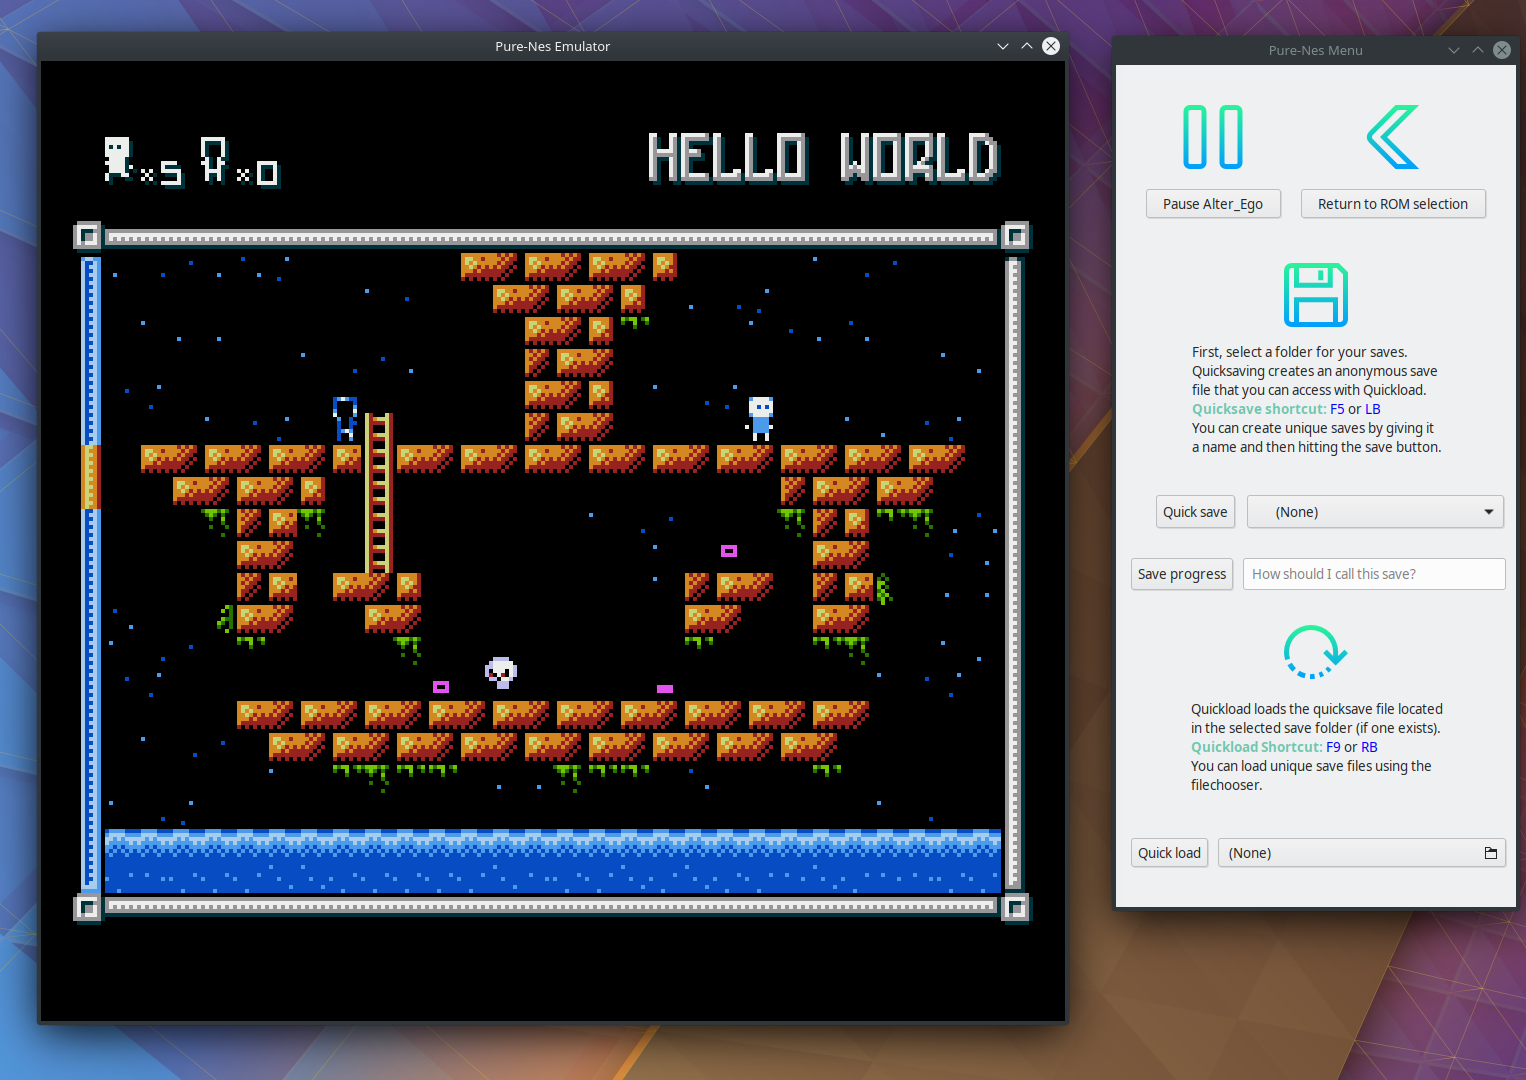
\includegraphics[scale=0.38]{shiru.png}
	\caption{Alter Ego. Linkért lásd: \ref{alter}}
	\vspace{1cm}
	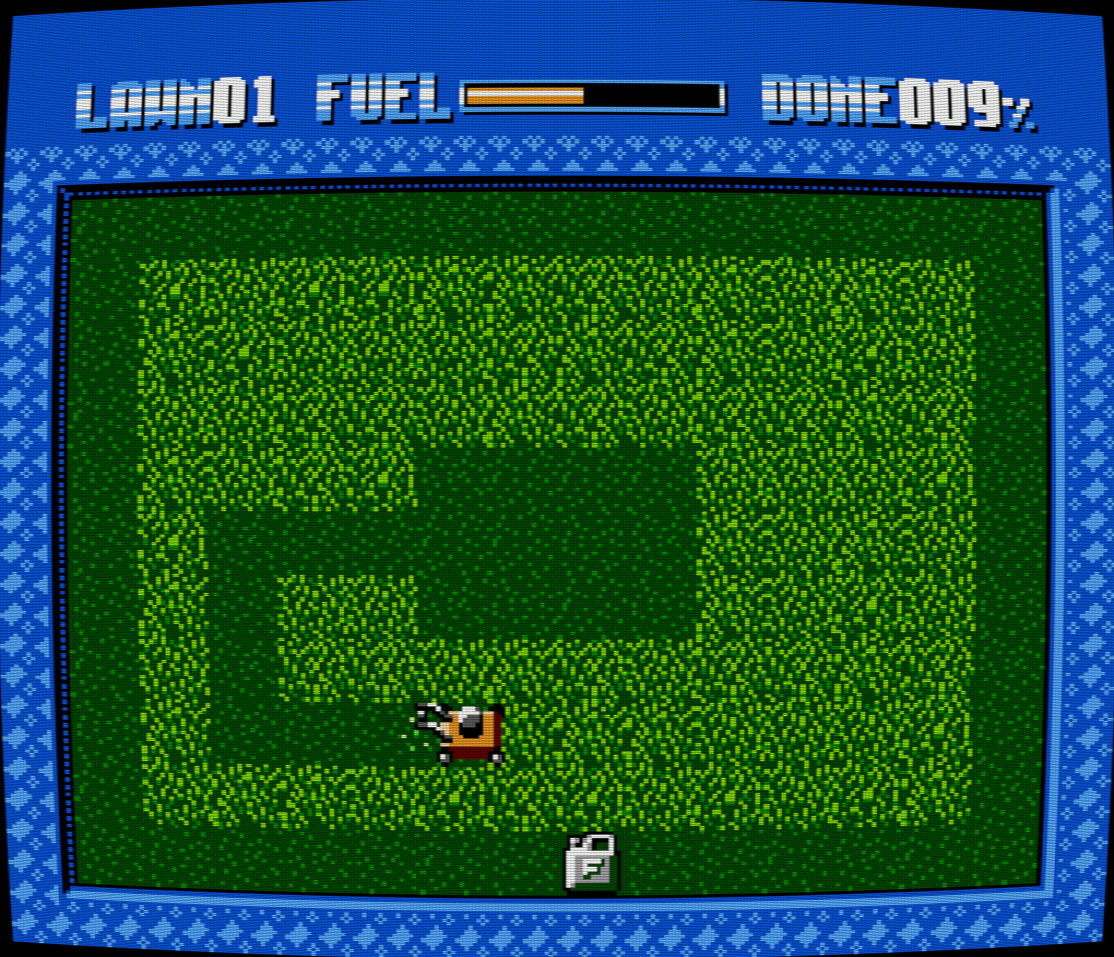
\includegraphics[scale=0.38]{lawn.png}
	\caption{Lawn Mover. Linkért lásd: \ref{lawn}}
\end{figure}